\chapter{Relation to Other Transport Modeling Frameworks}
\label{ch:relation}
% ##################################################################################################################

\hfill \textbf{Author:} Andreas Horni

\begin{center} 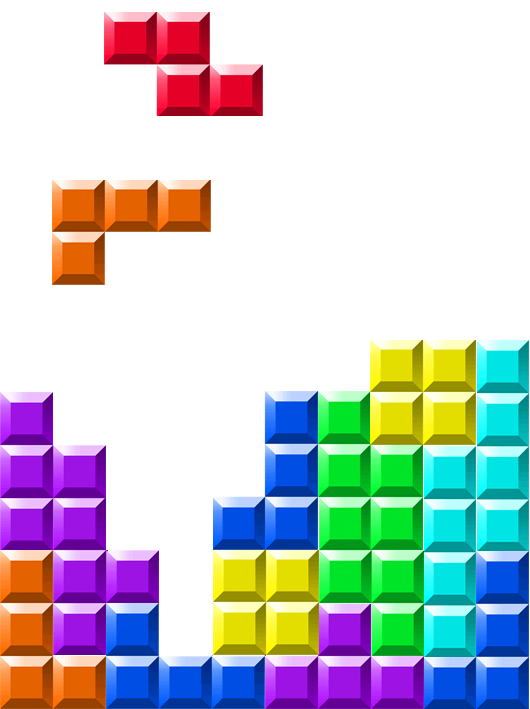
\includegraphics[width=0.3\textwidth, angle=0]{figures/MATSimBook.png} \end{center}

% ##################################################################################################################
a little theory hier unterbringen



\section{The 4-Step Procedure and Aggregate Forecasting Methods}
blablabla blablabla blablabla

blablabla blablabla

blablabla

% ##################################################################################################################
\section{Assignment Methods: Successors of Beckmann et al.}

% ##################################################################################################################
\section{Analytical and Other Numerical Methods (Variational Inequalities, Fixed Points)}

% ##################################################################################################################
\section{Other Microsimulation Frameworks}
\subsection{Rule-Based vs. Equilibrium-Based Frameworks}

(agent-based) microsims

% ##################################################################################################################
\section{Microsims in the Context of Different Types of Equilibria}
\label{sec:types}
% ------------------------------------------------------------------
\copied{\citet[][]{Horni_PhDThesis_2013}}

% ------------------------------------------------------------------
\textbf{Deterministic User Equilibrium (UE):}

% ------------------------------------------------------------------
\textbf{Stochastic User Equilibrium (SUE):}
 
% ------------------------------------------------------------------
\textbf{Dynamic User Equilibrium (DUE):}

% ------------------------------------------------------------------
\subsection{Existence, Uniqueness, Stability and Behavioral Basis of Equilibria}
For microsimulations, very little is known about the targeted equilibria. These models are highly dynamic, stochastic and disaggregate with many user classes and behaviorally rich decision principles. In Section \ref{sec:MATSimEquilibrium}, the MATSim equilibrium is discussed. As, in general, for the interpretation of results but also for model development (see equilibration discussion in Section \ref{sec:equilibration}), knowledge about the characteristics of the equilibrium searched is helpful, further research is strongly suggested.


\todo{
Gunnar \\
Daniel R. Leeds
}

% ##################################################################################################################